\chapter{XBee}
\label{chap:xbee}

%%%%%%%%%%%%%%%%%%%%%%%%%%%%%%%%%%%%%%%%%%%%%%%%%%%%%%%%%%%%%%%%%%%%%%%%%%%%%%%%
% Objetivo: Exponer la tecnología XBee                                         %
%%%%%%%%%%%%%%%%%%%%%%%%%%%%%%%%%%%%%%%%%%%%%%%%%%%%%%%%%%%%%%%%%%%%%%%%%%%%%%%%

\lettrine{N}{este} apéndice exponse todo o relacionado coa tecnoloxía
\textit{XBee}. \\

\textbf{XBee} \cite{XBee} é o nome comercial de \textit{Digi International}
para unha familia de módulos de radio con formato compatible. As primeiras
radios \textit{XBee} comercializáronse baixo a marca \textit{MaxStream} en 2005
e estaban baseados no estándar IEEE 802.15.4-2003, deseñado para comunicacións
punto a punto e en estrela e velocidades de transmisión sen fíos de 250 Kbps. \\

Inicialmente comercializáronse dous modelos, o \textit{XBee} de 1 mW e baixo
custe e o \textit{XBee-PRO} de 100 mW. Desde a comercialización inicial,
introduciuse no mercado unha nova serie de radios XBee e agora todas se venden
baixo a marca Digi. \\

As radios XBee precisan dun mínimo de catro conexións para ser usadas:
alimentación (3,3 V), terra e entrada e saída de datos (UART), sendo
recomendado tamén o uso de liñas Reset e Sleep. Ademais, a maioría das familias
XBee contan con algunhas liñas de control de fluxo, I/O, A/D e de sinalización
integradas. A versión programable do XBee conta cun procesador adicional para
código de usuario.

A familia de radios XBee componse de (figura \ref{figura:FamiliaXbee}):

\begin{figure}[htbp]
 \centering
 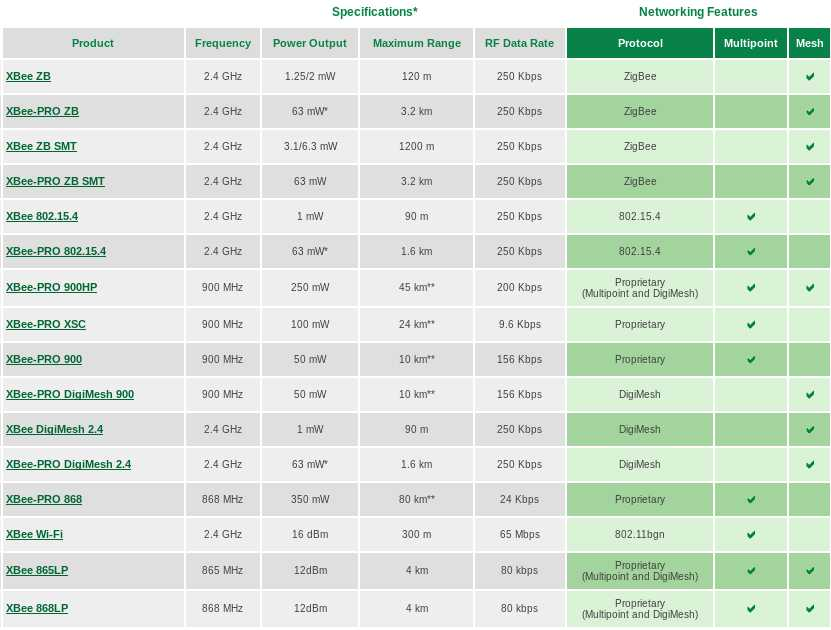
\includegraphics[scale=0.5,keepaspectratio=true]{./imagenes/familia-xbee.png}
 % familia-xbee.png: 831x630 pixel, 72dpi, 29.32x22.23 cm, bb=0 0 831 630
 \caption{Familia XBee \cite{XBee}}
 \label{figura:FamiliaXbee}
\end{figure}

\section{Formatos, antenas e modos de datos}

Os módulos XBee está dispoñibles en dous formatos de montaxe:
\textit{Through-Hole} e \textit{Surface Mount}. \\

Todos os modelos de XBee (a excepción do \textit{XBee 868LP}) no popular
formato Through-Hole de 20 pins. Certos módulos están tamén dispoñibles en
formato Surface Mount de 37 pads, formato popular en productos de alta demanda
debido ós reducidos custos da tecnoloxía SMT. \\

Os módulos XBee veñen normalmente con varias opcións de antena, incluíndo
\textit{U.FL}, \textit{PCB Embedded}, \textit{Wire} e \textit{RPSMA}. \\

Os módulos XBee poden traballar en modo de datos transparente ou en modo API
baseado en paquetes. No modo transparente, os datos dispoñibles no pin Data IN
(DIN) transmítense directamente e sen fíos ós módulos receptores sen
modificación ningunha. Os paquetes entrantes poden ser direccionados a un
obxectivo (punto a punto) ou repetilos a múltiples obxectivos (estrela). Este
modo emprégase principalmente en casos no que o protocolo existente non tolera
cambios no formato de datos. Para configurar un módulo empréganse comandos AT.
En modo API os datos son empaquetados permitindo o direccionamento, a
configuración de parámetros e o control de recepción de paquetes, incluíndo a
teledetección e o control dos pins dixitais de E/S e os pins de entrada
analóxicos.

\section{XBee ZB}

Os módulos Zigbee, XBee e XBee-PRO ZB (figura \ref{figura:XBeeZB-2},
proporcionan conectividade sen fíos de baixo custo a dispositivos de redes
ZigBee en malla (mesh).

\begin{figure}[htbp]
 \centering
 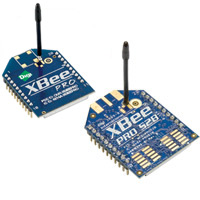
\includegraphics[scale=0.6,keepaspectratio=true]{./imagenes/xbee-zb.jpg}
 % xbee-zb.jpg: 200x200 pixel, 72dpi, 7.06x7.06 cm, bb=0 0 200 200
 \caption{XBee ZB}
 \label{figura:XBeeZB-2}
\end{figure}

\section{ZigBee}

\textbf{Zigbee} é o nome da especificación dun conxunto de protocolos de
comunicación sen fíos de alto nivel para a súa utilización en radiodifusión
dixital de baixo consumo, baseada no estándar \textit{IEEE 802.15.4} de redes
sen fíos de área persoal (WPAN). O seu obxectivo son as aplicacións que
requiren de comunicacións seguras con baixa taxa de envío de datos e
maximización da vida útil das súas baterías. \\

A tecnoloxía definida pola especificación de ZigBee está deseñada para ser máis
simple e menos custosa que outras WPAN, coma Bluetooth ou Wi-Fi. \\

As redes ZigBee están securizadas a través do uso de claves de cifrado
simétrico de 128 bits. As distancias de transmisión van desde os 10 ós 100
metros, dependendo da potencia de saída e das características ambientais. \\

ZigBee foi concebido en 1998, estandarizado en 2003 e revisado en 2006. O nome
refírese á danza das abellas.

 \subsection{Visión xeral}

 ZigBee é un estándar para redes en malla sen fíos de baixo consumo e baixo
 custe. O baixo custe permite que a tecnoloxía sexa empregada de forma masiva
 en aplicacións de control e monotorización sen fíos. O baixo consumo permite
 máis autonomía con baterías máis pequenas. As redes mesh proporcionan alta
 fiabilidade e un rango máis extenso. \\

 ZigBee opera nas bandas de radio industriais, científicas e médicas (ISM):
 868 MHz en Europa, 915 MHz en USA e Australia e 2,4 GHz na maior parte do
 mundo. A velocidade de transmisión varía desde os 20 Kbps na banda de
 frecuencia dos 868 MHz ata os 250 Kbps na banda de frecuencia dos 2,4 GHz. \\

 A capa de rede de ZigBee soporta nativamente tanto redes en árbore como en
 estrela, ademais de redes en malla xenéricas. Cada rede debe ter un
 dispositivo coordinador, encargado da súa creación, o control dos seus
 parámetros e o mantemento básico. En redes en estrela, o coordinador debe ser
 o nodo central. As redes en árbore e en malla permiten o uso de routers ZigBee
 para extender a comunicación a nivel de rede.

 ZigBee está construído sobre a capa física e a de control de acceso ó medio do
 estándar IEEE 802.15.4-2003 para redes WPAN de baixo taxa de transmisión. A
 especificación pretende completar o estándar engadindo catro compoñentes
 principais: a capa de rede, a capa de aplicación, os denominados
 \textit{ZigBee device objects} (ZDOs)e os
 \textit{manufacturer-defined application objects} que permiten a
 personalización en favor da integración total. \\

 Ademais de engadir dúas capas de rede de alto nivel para a estrutura
 subxacente, a mellora máis significativa é a introdución de ZDOs. Estes son
 os responsables dunha serie de tarefas, que inclúen o mantemento dos roles dos
 dispositivos, a xestión das solicitudes para participar nunha rede, a
 detección de dispositivos e a seguridade. \\

 ZigBee non pretende soportar \textit{powerline networking} pero si interactuar
 con el para propósitos de polo menos de medición intelixente e aplicacións
 intelixentes. \\

 Porque os nodos ZigBee poden pasar de estado de reposo a estado activo en
 30 ms ou menos, a latencia pode ser baixa e os dispositivos poden chegar a
 responder sen problemas. Se o comparamos cos retardos de Bluetooth desde
 estado de reposo a activo, que normalmente andan en torno ós 3 segundos, vemos
 unha gran diferencia. Ademais, os nodos ZigBee poden estar en modo de reposo a
 maior parte do tempo, polo que a media de consumo pode ser baixa, resultando
 nunha longa autonomía.

 \subsection{Historia}

 As redes de tipo ZigBee empezaron a ser concebidas sobre 1999, cando moitos
 instaladores se deron conta de que tanto Wi-Fi coma Bluetooth ían ser
 inusables para moitas aplicacións. Máis concretamente, moitos enxeñeiros viron
 a necesidade de redes de radio dixital ad-hoc auto-organizadas. A necesidade
 real das mallas leva sendo posta en dúbida desde aquelas, dada a súa longa
 ausencia no mercado.

  \subsubsection{ZigBee 2004}

  O estándar IEEE 802.15.4-2003 completouse en maio de 2003. \\

  No verán de 2003, \textit{Philips Semiconductors}, un grande contribuidor ás
  redes malladas, cortou a súa inversión. Sen embargo,
  \textit{Philips Lighting} continuou a participación de \textit{Philips}, polo
  que este continúa sendo membro promotor no
  \textit{ZigBee Alliance Board of Directors}. \\

  A \textit{ZigBee Alliance} anunciou en outubro de 2004 que a cantidade dos
  seus membros se dobraran e que eran xa máis de 100 compañías en 22 países. En
  abril de 2005 chegaron ás 150 compañías e en decembro de 2005 pasaron das
  200. \\

  A especificación de ZigBee foi ratificada o 14 de decembro de 2004. A
  \textit{ZigBee Alliance} anunciou a dispoñibilidade da especificación 1.0 o
  13 de xuño de 2005, coñecida como \textit{ZigBee 2004}.

  \subsubsection{ZigBee 2006}

  En setembro de 2006, anunciouse a especificación \textit{ZigBee 2006}. A pila
  do protocolo de 2004 está agora máis ou menos obsoleta. \\

  A versión de 2006 reempraza principalmente a estructura
  \textit{Message/Key Value Pair} usada na de 2004 cunha
  \textit{cluster library}.

  \subsubsection{ZigBee PRO}

  En 2007 publicouse unha nova versión, de nome \textit{ZigBee PRO}, tamén
  chamada \textit{ZigBee 2007} por veces. \\

  ZigBee PRO é totalmente compatible cos dispositivos ZigBee 2006. Un
  dispositivo ZigBee 2007 debe ser capaz de conectarse e operar nunha rede
  ZigBee 2006 e viceversa. Debido a diferencias no enrutado:

  \begin{itemize}
   \item Os dispositivos ZigBee PRO deben converterse en
         \textit{ZigBee End-Devices} (ZEDs) non enrutadores, nunha rede ZigBee
         2006.
   \item Os dispositivos ZigBee 2006 deben converterse en ZEDs nunha rede
         ZigBee PRO.
  \end{itemize}

  As aplicacións que se executan nestes dispositivos funcionan da mesma
  maneira, independentemente do perfil de pila que teñan por debaixo. \\

  O primeiro \textit{ZigBee Application Profile}, o \textit{Home Automation},
  foi publicado o 2 de novembro de 2007.

 \subsection{Usos}

 O protocolo ZigBee está pensado para aplicacións integradas que requiren
 baixo envío de datos e baixo consumo. A rede resultante usará moi pouca
 cantidade de enerxía. Os dispositivos individuais deben ter unha autonomía de
 polo menos dous anos para pasar a certificación ZigBee. \\

 As áreas típicas de aplicación inclúen:

 \begin{itemize}
  \item Entretemento no fogar e domótica: automatización, iluminación
        intelixente, control avanzado de temperatura, seguridade, audio e
        vídeo.
  \item Redes de sensores sen fíos.
  \item Control industrial.
  \item Sensores embebidos.
  \item Recolección de datos médicos.
  \item Alarmas de fumes e seguridade.
  \item Inmótica.
 \end{itemize}

\section{Estándar e perfís}

A \textit{ZigBee Alliance} é un grupo de compañías que manteñen e publican o
estándar ZigBee. O termo ZigBee é unha marca rexistrada deste grupo, non só un
estándar técnico. A Alliance publica perfís de aplicación que permiten a moitos
vendedores OEM crear productos interoperables. A relación entre IEEE 802.15.4 e
ZigBee é similar á que hai entre IEEE 802.11 e a
\textit{Wi-Fi Alliance}.

 \subsection{Licencia}

 Para propósitos non comerciais, a especificación ZigBee é gratuíta para
 tódolos públicos. A membresía de entrada á \textit{ZigBee Alliance}, chamada
 \textit{Adopter}, ofrece o acceso ás especificacións todavía non publicadas e
 o permiso para crear productos comerciais empregando as especificacións. \\

 \subsection{Perfís de aplicación}

 \begin{itemize}
  \item Especificacións publicadas:
        \begin{itemize}
         \item ZigBee Home Automation 1.2
         \item ZigBee Smart Energy 1.1b
         \item ZigBee Telecommunication Services 1.0
         \item ZigBee Health Care 1.0
         \item ZigBee RF4CE – Remote Control 1.0
         \item ZigBee RF4CE – Input Device 1.0
         \item ZigBee Light Link 1.0
         \item ZigBee IP 1.0
         \item ZigBee Building Automation 1.0
         \item ZigBee Gateway 1.0
         \item ZigBee Green Power 1.0 as optional feature of ZigBee 2012
        \end{itemize}
  \item Especificacións en desenvolvemento:
        \begin{itemize}
         \item ZigBee Smart Energy 2.0
         \item ZigBee Retail Services
         \item ZigBee Smart Energy 1.2/1.3
         \item ZigBee Light Link 1.1
         \item igBee Home Automation 1.3
        \end{itemize}
 \end{itemize}

\section{Hardware de comunicacións RF}

O deseño do radio usado por ZigBee foi cuidadosamente optimizado para o baixo
custo en producción a gran escala. Ten só unhas poucas fases analóxicas e
emprega circuítos dixitais onde é posible. \\

Aínda que os propios radios son baratos, o
\textit{ZigBee Qualification Process} implica unha validación completa dos
requisitos da capa física. Toda radio derivado do mesmo
\textit{validated semiconductor mask set} gozará das mesmas características RF.
Unha capa física non certificada que funcione mal podería arruinar a autonomía
doutros dispositivos nunha rede ZigBee. Os radios ZigBee teñen restriccións moi
axustadas sobre consumo e ancho de banda. \\

Este estándar especifica a operación nas bandas ISM dos 2,4 GHz (todo o mundo),
915 MHz (América e Australia) e 868 MHz (Europa). Na banda dos 2,4 GHz hai 16
canles asignadas, cada unha con 5 MHz de ancho de banda. Os radios usan
codificación de espectro ensanchado por secuencia directa, manexada polo fluxo
dixital dentro do modulador. Nas bandas de 868 e 915 MHz úsase modulación por
desprazamento de fase binaria (BPSK) e na banda dos 2,4 GHz úsase
\textit{offset quadrature phase-shift keying} (OQPSK) que transmite dous bits
por símbolo. \\

A velocidade de transmisión de datos en bruto (RAW) por canle é de 250 Kbps na
banda dos 2,4 GHz, 40 Kbps na de 915 MHz e 20 Kbps na de 868 MHz. A
transferencia de datos real será inferior á taxa de bits máxima especificada
debido á sobrecarga introducida pola paquetería e ós retardos de procesamento.
Para transmisións en interiores na banda dos 2,4 GHz o alcance pode ser de 10 a
20 metros, dependendo dos materiais de construcción, o número de paredes a
traspasar e da potencia legal de saída permitida. En exteriores e con visión
directa, o alcance pode ser de ata 1500 metros dependendo da potencia de saída
e das condicións ambientais. A potencia de saída dos radios é normalmente de
0-20 dBm (1-100 mW).

\section{Tipos de dispositivos e modos de operación}

Os dispositivos ZigBee poden ser de tres tipos:

\begin{itemize}
 \item \textit{ZigBee Coordinator} (ZC): o dispositivo máis completo, o
       \textit{Coordinator}, conforma a raíz da árbore de rede, puidendo facer
       de ponte a outras redes. Hai exactamente un ZC en cada rede que é o que
       creou a rede orixinalmente. Almacena información sobre a rede, incluíndo
       o actuar coma \textit{Trust Center} e repositorio de claves de
       seguridade.
 \item \textit{ZigBee Router} (ZR): ademais de executar funcións de
       aplicacións, un ZR pode actuar como intermediario pasando datos entre
       dispositivos.
 \item \textit{ZigBee End Device} (ZED): ten a funcionalidade xusta para
       comunicarse co nodo pai (a ZC or a ZR), pero non pode transmitir datos
       doutros dispositivos. Esta relación permite que o nodo esté durmido unha
       cantidade significativa do tempo, alongando a autonomía do dispositivo.
       Un ZED require a menor cantidade de memoria e, polo tanto é máis barato
       de fabricar ca un ZR ou un ZC.
\end{itemize}

O protocolo ZigBee soporta tanto redes con ou sen baliza. Nas redes sen baliza,
emprégase un mecanismo de acceso á canle de tipo CSMA/CA sen slot. Neste tipo
de redes, os ZR teñen tipicamente os seus receptores sempre activos, o que
require dunha fonte de alimentación máis potente. Sen embargo, isto permite
misturar nunha rede dispositivos heteroxéneos, onde uns reciben continuamente
mentres outros transmiten só cando detectan un estímulo externo. \\

Nas redes con baliza, os nodos especiais da rede (os ZR) transmiten balizas
periodicamente para confirmar a presencia doutros nodos. Os nodos poden durmir
entre balizas, extendendo a súa autonomía. O intervalo entre balizas depende da
velocidade de transmisión. Estará entre 15,36 ms e 251,65824 segundos a
250 Kbps, entre 24 ms e 393,216 segundos a 40 Kbps e entre 48 ms e 786,432 a
20 Kbps. Sen embargo, intervalos moi longos requiren alta precisión á hora de
medilos, o que pode entrar en conflicto cos baixos custes de producción. \\

En xeral, o protocolo ZigBee minimizan o tempo que o radio está encendido e,
por tanto, o consumo. En redes con balizas, os nodos só necesitan estar activos
cando se transmite unha baliza. En redes sen balizas, o consumo é asimétrico:
algúns dispositivos están sempre activos mentres outros están a maior parte do
tempo durmindo. \\

Excepto o \textit{Smart Energy Profile 2.0}, os dispositivos ZigBee teñen que
cumprir co protocolo estándar 802.15.4-2003
\textit{Low-Rate Wireless Personal Area Network} (LR-WPAN). O estándar
especifica as capas máis baixas do protocolo: a capa física (PHY) e a parte do
control de acceso ó medio da capa de enlace de datos (DLL). O modo básico de
acceso á canle é o \textit{carrier sense, multiple access/collision avoidance}
(CSMA/CA). É dicir, comproban que ninguén esté transmitindo antes de comezar a
transmitir, excepto en tres casos:

\begin{itemize}
 \item As balizas envíanse en intervalos fixos, polo que non usan CSMA.
 \item Os ACKs tampouco usan CSMA.
 \item As redes con balizas con requisitos de tempo real de baixa latencia usan
       \textit{Guaranteed Time Slots} (GTS), o cal, por definición, non usa
       CSMA.
\end{itemize}

\section{Software}

O software está deseñado para ser desenvolvido en procesadores pequenos e
baratos.

\begin{figure}[htbp]
 \centering
 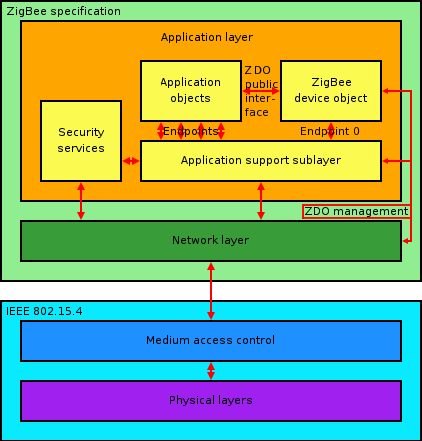
\includegraphics[scale=0.6,keepaspectratio=true]{./imagenes/zigbee-pila-protocolo.png}
 % zigbee-pila-protocolo.png: 422x441 pixel, 72dpi, 14.89x15.56 cm, bb=0 0 422 441
 \caption[ZigBee: pila do protocolo]{ZigBee: pila do protocolo \cite{ZigBeeProtocolStack}}
 \label{figura:ZigBeePilaProtocolo}
\end{figure}

 \subsection{Capa de rede}

 As funcións principais da capa de rede son habilitar o correcto uso da subcapa
 MAC e proporcionar unha interface adecuada para ser usada pola capa superior,
 a capa de aplicación. As súas capacidades e estructura son as típicas
 asociadas a outras capas de rede, incluíndo o enrutamento. \\

 Por unha banda, a entidade de datos crea e xestiona unidades de datos da capa
 de rede da carga útil da capa de aplicación e realiza o enrutamento de acordo
 coa topoloxía actual. \\

 Por outra, está o control de capa, que se usa para manexar a configuración de
 novos dispositivos e estableces novas redes: pode determinar se un dispositivo
 pertence á rede e detectar novos veciños e routers. O control tamén pode
 detectar a presenza dun receptor, o que permite comunicación directa e
 sincronización da MAC. \\

 O procotolo de enrutamento usado pola capa de rede é o \textit{AODV}. Coa fin
 de atopar o dispositivo de destino, transmite unha petición de ruta a todos os
 seus veciños e estes ós seus ata que chega ó seu destino. Unha vez que alcanza
 o destino, envía unha resposta de ruta a través dunha transmisión unicast
 seguindo a ruta con menor custe ata a fonte. Unha vez que a fonte recibe a
 resposta, esta actualiza a súa táboa de enrutamento para a dirección de destino
 co seguinte salto na ruta de acceso e o custe da ruta.

 \subsection{Capa de aplicación}

 A capa de aplicación é a capa de máis alto nivel definida pola especificación
 e é a interface do sistema ZigBee que empregarán os seus usuarios finais.
 Comprende a maioría dos compoñentes engadidos pola especificación ZigBee:
 tanto os ZDO coma os seus procedementos de xestión, xunto cos obxectos de
 aplicación definidos polo fabricante, son considerados parte desta capa.

 \subsection{Compoñentes principais}

 O ZDO é o responsable de definir o rol dun dispositivo coma coordinador ou
 dispositivo final, pero tamén de detectar os novos dispositivos da rede a
 distancia dun salto e identificar os servizos que ofrecen. É entón cando pode
 pasar a establecer enlaces seguros con dispositivos externos e responder
 adecuadamente ás peticións de enlace. \\

 A subcapa de soporte de aplicación (APS) é o outro compoñente estándar
 principal da capa e, como tal, ofrece unha interface ben definida e uns
 servizos de control. Funciona coma ponte entre a capa de rede e os outros
 compoñentes da capa de aplicación: mantén actualizadas as táboas de enlace en
 forma de base de datos, que poden ser usadas para atopar dispositivos
 apropiados dependendo dos servizos que sexan necesarios e do que ofrezan os
 diferentes dispositivos. Como a unión entre as dúas capas especificadas, tamén
 enruta a través das capas da pila do protocolo.

 \subsection{Modelos de comunicación}

 Unha aplicación pode consistir en comunicar obxectos que cooperan para
 realizar as tarefas desexadas. O foco de ZigBee é distribuír o traballo
 entre varios dispositivos diferentes que forman parte dunha rede ZigBee. \\

 A colección de obxectos que forman a rede comunícanse empregando as
 facilidades que ofrece APS, supervisados por interfaces ZDO. O servizo de
 datos da capa de aplicación segue unha estructura típica de
 \textit{request-confirm/indication-response}. Dentro dun único dispositivo
 poden existir ata 240 obxectos de aplicación, numerados dentro do rango 1-240.
 O 0 está reservado para interface de datos do ZDO e o 255 para o broadcast; o
 rango 241-254 está reservado para usos futuros. \\

 Hai dous servizos dispoñibles para ser usados polos obxectos de aplicación:

 \begin{itemize}
  \item O servizo \textit{key-value pair} (KVP) está destinado a propósitos de
        configuración. Habilita a descripción, petición e modificación de
        atributos de obxecto a través dunha simple interface baseada en
        funcións getters/setters e de eventos, algunhas das cales permiten unha
        petición por resposta. A configuración emprega XML comprimido (pódese
        usar tamén XML sen compresión) para proporcionar unha solución
        adaptable e elegante.
  \item O servizo de mensaxes está deseñado para ofrecer unha aproximación
        xeral para o tratamento da información, evitando a necesidade de
        adaptar os protocolos de aplicación e a potencial sobrecarga na que
        incorre o KVP. Permite que payloads arbitrarios sexan transmitidos en
        frames APS.
 \end{itemize}

 O direccionamento é tamén parte da capa de aplicación. Un nodo de rede
 componse dun radio transceptor conforme á especificación 802.15.4 e unha ou
 máis descripcións de dispositivo (basicamente coleccións de atributos que
 poden ser consultados ou configurados, ou monitorizados a través de eventos).
 O transceptor é a base para o direccionamento, e os dispositivos dentro dun
 nodo especifícanse mediante un identificador de punto final no rango 1-240.

 \subsection{Comunicación e detección de dispositivos}

 Para que as aplicacións poidan comunicarse, os dispositivos que comprenden
 deben usar un protocolo de aplicación común (tipos de mensaxes, formatos e
 demais); estes conxuntos de convencións agrúpanse en perfís. Ademais, o
 enlazado decídese emparellando os identificadores de clúster de entrada e
 saída, únicos dentro do contexto dun perfil dado e asociados a un fluxo de
 datos entrante ou saínte dun dispositivo. As táboas de enlazado conteñen pares
 de orixe e destino. \\

 En función da información dispoñible, a detección de dispositivos pode seguir
 diferentes métodos. Cando se coñece a dirección de rede, a dirección IEEE pode
 ser solicitada mediante comunicación unicast. En caso contrario, as peticións
 faranse mediante broadcast (a dirección IEEE será parte do payload de
 resposta). Os dispositivos finais responderán simplemente coa dirección
 solicitada, mentres un coordinador de rede ou router enviará tamén as
 direccións de todos os dispositivos asociados con el. \\

 Este protocolo de detección extendida permite os dispositivos externos sepan
 sobre os dispositivos dunha rede e os servizos que ofrecen, facilitando que os
 dispositivos finais desa rede poidan informar cando son solicitados polo
 dispositivo detector (o cal obtivo previamente as súas direccións). Os
 servizos que coincidan poden ser usados tamén. \\

 O uso de identificadores de clúster reforza o enlace de entidades
 complementarias por medio de táboas de enlace, que son mantidas polos
 coordinadores ZigBee, dado que as táboas deben estar sempre dispoñibles dentro
 dunha rede e os coordinadores son os máis propensos a ter unha fonte de
 alimentación permanente. As copias de seguridade, xestionadas por capas de
 alto nivel, poden ser necesarias para algunha aplicación. \\

 A comunicación pode ocorrer logo da asociación. O direccionamento directo usa
 tanto a dirección do radio coma o identificador do punto final, mentres que o
 direccionamento indirecto usa todo campo relevante (dirección, punto final,
 clúster e atributo) que precisan de ser enviados ó coordinador da rede, o cal
 mantén asociacións e peticións de traducción para a comunicación. O
 direccionamento indirecto é particularmente útil para manter algúns
 dispositivos moi sinxelos e minimizar a súa necesidade de almacenamento.
 Ademais destes dous métodos, está permitido facer broadcast a todos os puntos
 finais dun dispositivo e o direccionamento en grupo úsase para comunicarse con
 grupos de puntos finais pertencentes a un conxunto de dispositivos.

\section{Servizos de seguridade}

Como unha das súas características definidoras, ZigBee ofrece facilidades para
a realización de comunicacións seguras, protexendo o establecemento e
transporte de claves criptográficas, frames de cifrado e dispositivos de
control. Baséase no framework de seguridade básico definido en IEEE 802.15.4.
Esta parte da arquitectura depende da correcta xestión de claves simétricas e
da correcta implementación dos métodos e políticas de seguridade.

 \subsection{Modelo de seguridade básico}

 O mecanismo básico para asegurar a confidencialidade é a adecuada protección
 de todo o material relacionado coas claves. A confianza debe ser asumida na
 instalación inicial das claves, así coma no procesamento da información de
 seguridade. Para que unha implementación funcione a nivel global, asúmese que
 o seu comportamento é conforme ó especificado. \\

 As claves son a pedra angular da arquitectura de seguridade; como tal a súa
 protección é de suma importancia, e as claves nunca deben ser transportadas a
 través dunha canle insegura. Unha excepción momentánea a esta regra ocorre
 durante a fase inicial de adición á rede dun dispositivo non configurado
 anteriormente. O modelo de rede de ZigBee debe ter especial coidado das
 consideracións de seguridade, como rede ad hoc debe ser fisicamente accesible
 a dispositivos externos pero o ambiente de traballo particular non pode ser
 predito; de igual xeito, as distintas aplicacións correndo simultaneamente e
 utilizando o mesmo transceptor para comunicarse deben ser mutuamente
 confiables: por razóns de custo, o modelo asume que non hai un firewall entre
 entidades de nivel de aplicación. \\

 Dentro da pila do protocolo, as diferentes capas de rede non están
 criptograficamente separadas, polo que son necesarias políticas de acceso e se
 asume un deseño correcto. O modelo de confianza aberto dentro dun dispositivo
 permite compartir claves, o que reduce os custos notablemente. Con todo, a
 capa que crea un frame é responsable da súa seguridade. Se puidesen existir
 dispositivos maliciosos, todo payload da capa de rede debe ser cifrado, de
 maneira que todo tráfico non autorizado poida ser inmediatamente rexeitado. A
 excepción, unha vez máis, é a transmisión da clave de rede (que confire unha
 capa de seguridade unificada á rede) a un novo dispositivo de conexión.

 \subsection{Arquitectura de seguridade}

 ZigBee usa claves de 128 bits para implementar os seus mecanismos de
 seguridade. Unha clave pode ser asociada a unha rede (sendo usable por ambas
 capas ZigBee e a subcapa MAC) ou a un enlace, adquirida a través dunha
 pre-instalación, acordo ou transporte. O establecemento de claves de enlace
 baséase nunha clave mestra que controla a correspondencia entre claves de
 enlace. En último caso, alomenos a clave mestra de inicio debe ser obtida a
 través dun medio seguro (transporte ou pre-instalación), dado que a seguridade
 de toda a rede depende dela. As claves mestras e de enlace só son visibles
 pola capa de aplicación. Diferentes servizos usan diferentes variacións de
 sentido único da clave de enlace a fin de evitar perdas e riscos de
 seguridade. \\

 A distribución de claves é unha das funcións máis importantes da rede. Unha
 rede segura designará un dispositivo especial no que os demáis dispositivos
 confiarán para a distribución de claves seguras: o \textit{Trust Center}.
 Idealmente, os dispositivos terán a dirección do Trust Center e a clave mestra
 inicial precargadas; se se permite un momento de vulnerabilidade, será enviada
 como se describiu anteriormente. As aplicacións típicas sen necesidades
 especiais de seguridade usarán unha clave de rede proporcionada polo Trust
 Center (a través da canle insegura inicial) para comunicarse. \\

 Así, o Trust Center mantén a clave de rede e proporciona seguridade punto a
 punto. Os dispositivos só aceptarán comunicacións orixinadas a partir dunha
 clave proporcionada polo Trust Center, excepto para a clave mestra inicial. A
 arquitectura de seguridade está distribuída entre as capas de rede como segue:

 \begin{itemize}
  \item A subcapa MAC é capaz de facer comunicacións fiables dun só salto. Como
        regra xeral, o nivel de seguridade a empregar será especificado polas
        capas superiores.
  \item A capa de rede controla o enrutamento, o procesamento das mensaxes
        recibidas e o ser capaz de facer broadcast das peticións. Os frames de
        saída usarán a clave adecuada acorde á ruta, se está dispoñible; noutro
        caso, usarase a clave de rede para protexer o payload de dispositivos
        externos.
  \item A capa de aplicación ofrece servizos de establecemento de claves e de
        transporte tanto ó ZDO como ás aplicacións. É tamén responsable da
        propagación a través da rede dos cambios nos dispositivos que a
        compoñen, que poden ter orixe nos propios dispositivos (por exemplo, un
        simple cambio de estado) ou no Trust Manager (que pode informar á rede
        de que un certo dispositivo vai ser elimidado da mesma). Tamén enruta
        as peticións desde os dispositivos ó Trust Center e as renovacións da
        clave de rede desde o Trust Center a tódolos dispositivos. Ademais
        disto, o ZDO mantén as políticas de seguridade do dispositivo.
 \end{itemize}

 A infrastructura de niveles de seguridade está baseada en CCM*, que engade
 funcionalidades de cifrado e integridade a CCM.
